\documentclass{article}

\usepackage{authblk}  % author affiliation
\usepackage{amsmath}  % math stuff
\usepackage[dashed=false, sorting=none, style=ieee]{biblatex}  % bibliography
\usepackage{graphicx}  % eps plots and figures
\usepackage[utf8]{inputenc}
\usepackage[letterpaper, portrait, margin=1in]{geometry}  % adjust paper size, margin
\usepackage{indentfirst}  % always indent paragraph

\addbibresource{references.bib}  % bibliography

\title{Piecewise hierarchical implicit surface structures constructed using tetrahedron-based unit cells}
\author[1]{Ruiqi Chen\thanks{rchensix@alumni.stanford.edu}}
\author[1]{Hardik Kabaria\thanks{hardik@carbon3d.com}}
\author[1]{Saigopal Nelaturi\thanks{snelaturi@carbon3d.com}}
\author[2]{Adrian Lew\thanks{lewa@stanford.edu}}
\affil[1]{Carbon Inc., 1089 Mills Way, Redwood City CA 94063}
\affil[2]{Department of Mechanical Engineering, Stanford University, 440 Escondido Mall, Stanford CA 94305}
\date{}

\begin{document}

\maketitle

\begin{abstract}
   Additive manufacturing enables the creation of physical structures that cannot be manufactured using any other technique. This work introduces a new methodology to create complex lattice structures that can be additively manufactured for various applications, including energy absorption and biomedical scaffolding. First, an implicit surface is generated using a trigonometric 3D Fourier series. The Fourier series terms are carefully chosen such that the resulting implicit surface has full tetrahedral symmetry at particular points. Second, a tetrahedron-based unit cell is then isolated from the implicit surface by performing a boolean intersection between the implicit surface and a carefully placed regular tetrahedron. Possible locations and orientations for the placement of the regular tetrahedron are provided. Third, a tetrahedron mesh of a design space is generated using one of various techniques. Finally, the tetrahedron-based unit cell is then mapped via an affine transformation to every tetrahedron in a tetrahedron mesh, creating a piecewise lattice structure. A variety of tetrahedron-based unit cells may be used, greatly opening up the design space of lattice structures. While similar techniques have been demonstrated by mapping cubic unit cells to hexahedron meshes, they cannot be easily automated due to the difficulty in generating conformal hexahedron meshes. On the other hand, the methodology presented here only uses tetrahedron meshes, allowing it to be automated for purposes of topology optimization and inverse design.
\end{abstract}

Keywords: implicit surface, tetrahedron, symmetry, lattice, mesh, additive manufacturing, triply periodic minimal surface

\section{Introduction}

\section{Literature Review}

\section{Methodology}
Tetrahedron-based unit cell stencils are generated by first constructing an implicit surface cubic stencil using a 3D Fourier series. The terms of the Fourier series are carefully chosen such that the cubic stencil possesses achiral tetrahedral symmetry. The tetrahedron-based unit cell stencil is then isolated by taking the intersection a properly oriented regular tetrahedron with the implicit surface. To generate the lattice structure, a tetrahedron mesh of the input domain is created using an appropriate algorithm. Finally, the unit cell stencil is mapped to each tetrahedron in the mesh through an affine transformation, creating a piecewise implicit surface lattice structure. A brief overview of tetrahedral symmetry, space groups, and implicit surfaces is provided before proceeding to the lattice structure generation procedure.

\subsection{Symmetry considerations}
A regular tetrahedron with no markings or coloring possesses achiral (or full) tetrahedral symmetry, denoted as $T_d$. The symmetry group $T_d$ is comprised of the identity, four 3-fold rotational symmetry axes, three 2-fold rotational symmetry axes (which are also 4-fold rotoinversion symmetry axes), and six mirror planes, yielding a symmetry order of 24. The rotational axes, rotoinversion axes, and mirror planes of a regular tetrahedron are depicted in Figure \ref{fig:achiral_tetrahedron_symmetry}.
\begin{figure}
    \centering
    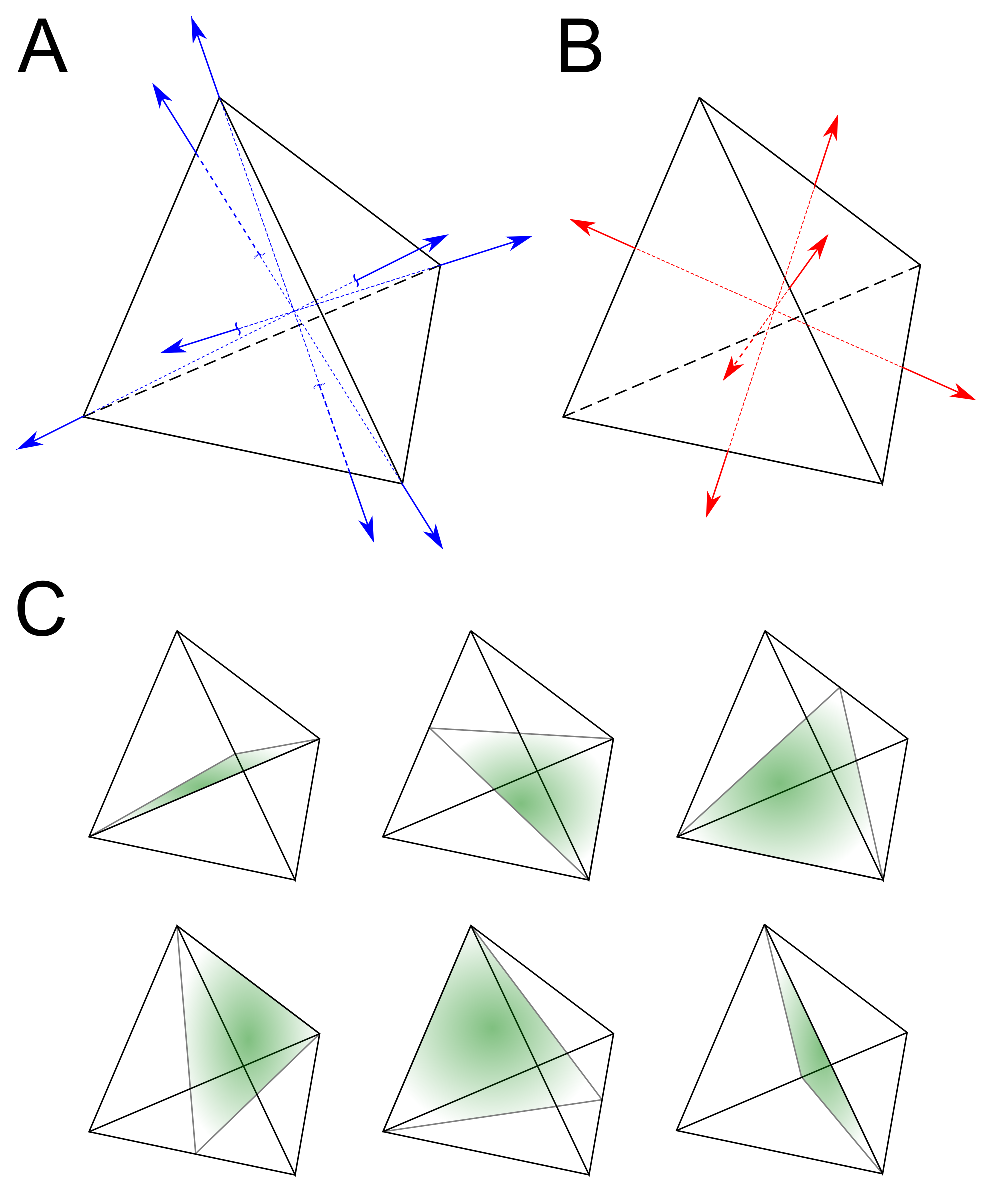
\includegraphics[width=0.5\linewidth]{figures/achiral_tetrahedron_symmetry.eps}
    \caption{Achiral tetrahedral symmetry $T_d$. Depicted are (a) four 3-fold rotational symmetry axes, (b) three 4-fold rotoinversion symmetry axes (which are also 2-fold rotational symmetry axes), and (c) six mirror symmetry planes.}
    \label{fig:achiral_tetrahedron_symmetry}
\end{figure}
On the other hand, a chiral tetrahedron possesses chiral tetrahedral symmetry, denoted as $T$. The symmetry group $T$ is a subgroup of $T_d$ and is comprised of only the rotational symmetries of $T_d$, yielding a symmetry order of 12 (i.e. no reflections or rotoinversions). Two chiral tetrahedrons and an achiral tetrahedron are depicted in Figure \ref{fig:chiral_achiral_tetrahedron}.
\begin{figure}
    \centering
    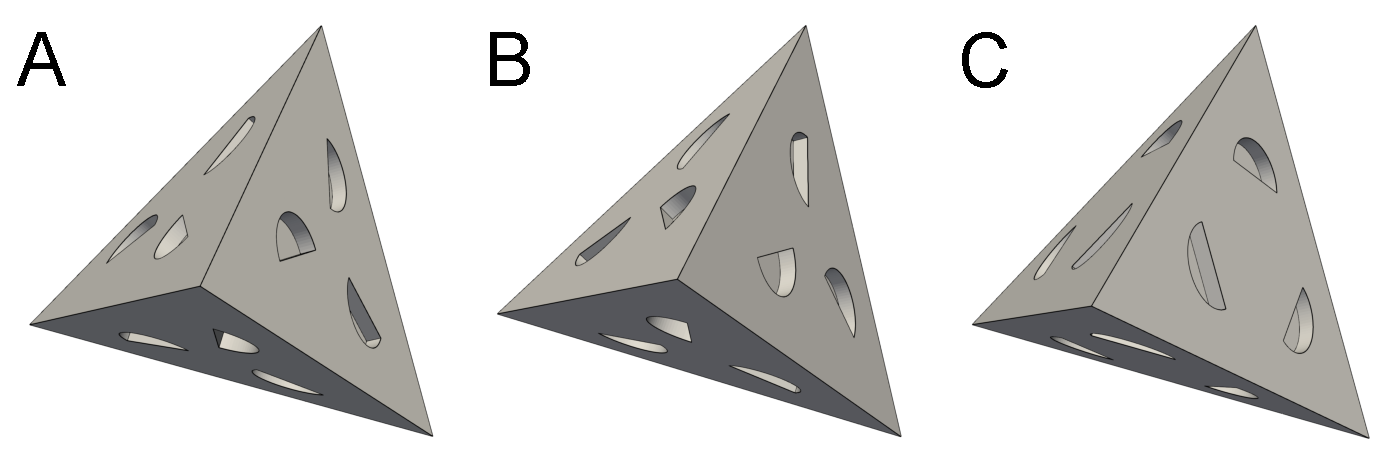
\includegraphics[width=0.5\linewidth]{figures/chiral_achiral_tetrahedron.eps}
    \caption{(A) Chiral tetrahedron with clockwise hole pattern. (B) Chiral tetrahedron with counterclockwise hole pattern. (C) Achiral tetrahedron.}
    \label{fig:chiral_achiral_tetrahedron}
\end{figure}
If two tetrahedrons of the type shown in Figure \ref{fig:chiral_achiral_tetrahedron}A are arranged such that their faces join together, the holes on the faces would be partially covered up due to the chirality. However, if two achiral tetrahedrons of the type shown in Figure \ref{fig:chiral_achiral_tetrahedron}C are arranged in the same way, the holes would not be covered up. Because this work is interested in joining together tetrahedron-based unit cells to create a lattice structure, the unit cells should have $T_d$ symmetry to allow faces to join without obscuring features.

To find tetrahedron-based unit cells with $T_d$ symmetry, this works looks at a related family of periodic space filling structures based on a cubic unit cell. All periodic structures (cubic or otherwise) can be categorized into space groups. A space group consists of the set of transformations, or symmetry operations, that, when applied to an object that belongs to that space group, produces the same object. Unlike the point groups $T$ and $T_d$ (which keep a center point fixed in space), space groups also include additional symmetry operations such as translations, glide planes, and screw axes. For periodic structures, there are 230 distinct crystallographic space groups. Each space group is assigned a number and the set of transformations for each space group are tabulated in the International Tables for Crystallography (ITC) \cite{hahn1983international}. Out of the 230 space groups, there are a handful that possess $T_d$ symmetry: 215 ($P\overline{4}3m$), 216 ($F\overline{4}3m$), 217 ($I\overline{4}3m$), 221 ($Pm\overline{3}m$), 224 ($Pn\overline{3}m$), 225 ($Fm\overline{3}m$), 227 ($Fd\overline{3}m$), and 229 ($Im\overline{3}m$). These space groups are all part of the cubic crystal system. By using a cubic unit cell from one of these space groups as the starting point, a tetrahedron-based unit cell with $T_d$ symmetry can be derived from the cubic unit cell. While theoretically any cubic unit cell from one of these space groups can be used, this work is interested in cubic unit cells generated by implicit equations in the form of a 3D Fourier series, as these have been shown to produce lightweight sheet-like and skeletal-like lattice structures.

\subsection{Periodic implicit surfaces constructed using 3D Fourier series}
\label{sec:fourier}

An implicit surface is a surface in 3D defined by the equation $f(x, y, z) = 0$. All points that satisfy the equation are located on the surface. Some examples of implicit surfaces include $f(x, y, z) = x^2 + y^2 + z^2 - r^2$ (representing a origin-centered sphere with radius $r$) and $f(x, y, z) = cos(x) + cos(y) + cos(z)$ (an approximation to the Schwarz primitive minimal surface). Implicit surfaces partition space into interior and exterior regions depending on the sign of the function $f(x, y, z)$ at a given point in space. This work uses the convention that interior points take on negative values. Implicit surfaces can also be defined in non-Euclidian space such as hyperbolic space, but this work only considers them in Euclidian space.

Periodic implicit surfaces can be constructed as a sum of trigonometric functions, representing a 3D Fourier series. The general form is given by
\begin{equation}
    \label{eq:fourier}
        f(x, y, z) = \sum\limits_{h,k,l} c_{hkl} f_{hkl}(x, y, z)
\end{equation}
where
\begin{equation}
    \begin{split}
        f_{hkl} & = e^{2\pi i\left(\frac{hx}{l_x}+\frac{ky}{l_y}+\frac{lz}{l_z}\right)} \\
        & = \cos{\left(2\pi \left(\frac{hx}{l_x}+\frac{ky}{l_y}+\frac{lz}{l_z}\right)\right)} + i \sin{\left(2\pi \left(\frac{hx}{l_x}+\frac{ky}{l_y}+\frac{lz}{l_z}\right)\right)}
    \end{split}
\end{equation}
and $h$, $k$, $l$ are positive integers, $l_x$, $l_y$, and $l_z$ are lengths of the unit cell along the Cartesian $x$, $y$, $z$ directions, and $c_{hkl}$ are complex-valued weighting constants. Note that while Eq. \ref{eq:fourier} is in general complex-valued, either the real or imaginary part of Eq. \ref{eq:fourier} can be used to define the implicit surface. In addition, for cubic unit cells, $l_x = l_y = l_z = L$, so without loss of generality, $L$ can be set to unity.

To generate cubic unit cells of a particular space group, every symmetry operation from the chosen space group is applied to $f_{hkl}$, and the resulting transformed $f_{hkl}$ equations are summed up \cite{wohlgemuth2001triply}. For example, consider the cubic space group 215 $(P\overline{4}3m)$ with 24 symmetry operations $(x, y, z), (x, \overline{y}, \overline{z}), (\overline{x}, y, \overline{z}), ..., (\overline{y}, \overline{x}, z)$. Applying all 24 operations to $f_{hkl}$ and summing the terms yields
\begin{equation}
    \label{eq:group215}
    \begin{split}
        f_{hkl}^{(215)}(x, y, z) & = f_{hkl}(x, y, z) + f_{hkl}(x, -y, -z) + f_{hkl}(-x, y, -z) + ... f_{hkl}(-y, -x, z) \\
        & = e^{2\pi i \left( hx+ky+lz \right)} + e^{2\pi i \left( hx-ky-lz \right)} + e^{2\pi i \left(-hx+ky-lz \right)} + ... + e^{2\pi i \left(-hy-kx+lz \right)}
    \end{split}
\end{equation}
Equation \ref{eq:group215} can be used as the starting point to generate a cubic unit cell within space group 215 by choosing positive integer values of $h$, $k$, $l$. In addition, linear combinations of Equation \ref{eq:group215} with complex-valued weights $c_{hkl}$ will also produce a cubic unit cell within space group 215. Thus, the implicit surface equation for a cubic unit cell within space group 215 is given by
\begin{equation}
    \label{eq:group215_full}
    f^{(215)}(x, y, z) = \sum\limits_{h,k,l} c_{hkl} f_{hkl}^{(215)}(x, y, z)
\end{equation}
where either the real or imaginary part of Equation \ref{eq:group215_full} can be used to define the implicit surface. Analogous equations can be developed for any other space group, including non-cubic space groups, with appropriate choices of $l_x$, $l_y$, and $l_z$ (for certain lower-numbered space groups, skew coordinates may be necessary).

The implicit surface may also be modified by a constant offset parameter $t$, yielding a skeletal lattice \cite{al2018topology}:
\begin{equation}
    f_{skeletal} = f_{original} - t
\end{equation}
where $f_{original}$ refers to the implicit surface equation before offsetting, and $t$ is the offset amount. In general, $t$ may be positive or negative. To create a sheet-like implicit surface, an implicit equation can be offset in both directions by some constant $t$:
\begin{equation}
    \begin{split}
        f_{sheet} & = \left(f_{original} + t\right)\left(f_{original} - t\right) \\
        & = f_{original}^2 - t^2
    \end{split}
\end{equation}
Offsetting using this approach does not change the space group that the original implicit surface belongs to. The offset parameter $t$ is not exactly a thickness parameter, but changing it does cause various measures of thickness (e.g. minimum wall thickness, maximum wall thickness, etc.) to change. However, even if $t$ is constant, the change in thickness is likely not spatially uniform.

Implicit surfaces generated using this method can be used to model many famous geometries, such as approximations to triply periodic implicit surfaces (TPMS). Several TPMS approximations are depicted in Figure \ref{fig:cubic_lineup} along with their corresponding space groups. The research conducted by Wohlgemuth and associates \cite{wohlgemuth2001triply} used this method as a way to discover several new TPMS approximations, but this work is not concerned with whether a particular implicit surface is also a minimal surface approximation. Rather, \textit{any} implicit surface from the aforementioned space groups can be used to generate a tetrahedron-based unit cell, as long as the resulting tetrahedron unit cell is composed of a single connected component (for manufacturing reasons).

\begin{figure}
    \centering
    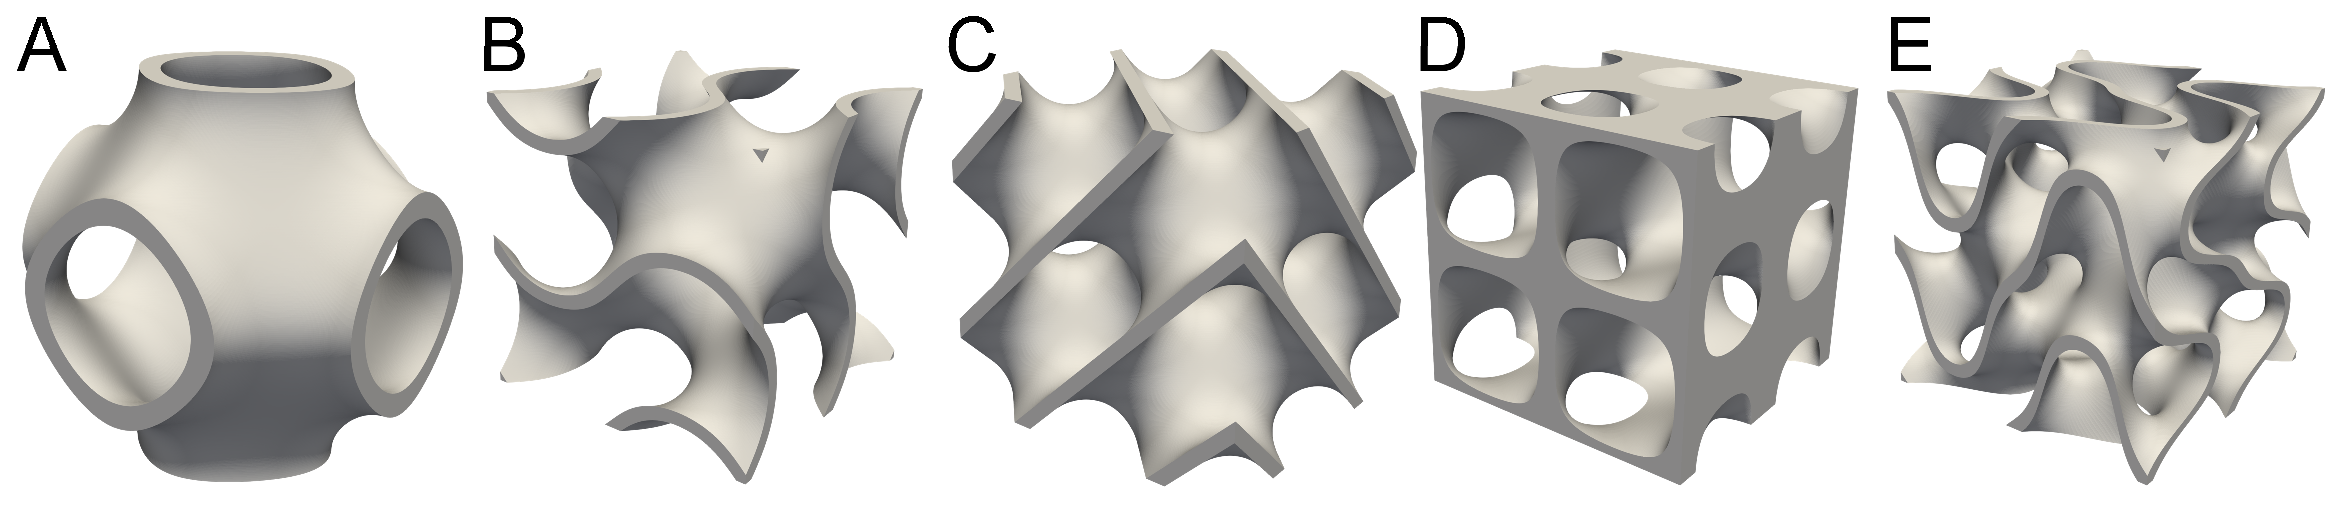
\includegraphics[width=\linewidth]{figures/cubic_lineup.eps}
    \caption{Collection of implicit surfaces that approximate triply periodic minimal surfaces. (a) Schwarz primitive ($Pm\overline{3}m$, no. 221), (b) gyroid ($I4_132$, no. 214), (c) diamond ($Fd\overline{3}m$, no. 227), (d) CLP ($P4_2/mcm$, no. 132), and (e) Fisher-Koch S ($Ia\overline{3}d$, no. 230).}
    \label{fig:cubic_lineup}
\end{figure}

\subsection{Generating the piecewise lattice structure}
\subsubsection{Tetrahedron-based unit cell}
The tetrahedron-based unit cell with $T_d$ symmetry is created by taking the intersection of the cubic unit cell (from one of the aforementioned space groups) with an appropriately oriented regular tetrahedron. The intersection operation can be done explicitly or implicitly. For the explicit intersection, the implicit surface of the cubic unit cell first needs to be triangulated using some appropriate method (e.g. marching cubes or marching triangles), then a boolean intersection operation can be performed on the explicit triangle meshes. For the implicit intersection, the regular tetrahedron must first be expressed as an implicit surface. This can be accomplished by considering the regular tetrahedron with vertices $\mathbf{p_1}$, $\mathbf{p_2}$, $\mathbf{p_3}$, $\mathbf{p_4}$ (in the order depicted in Figure \ref{fig:unit_tetrahedron}) as the intersection of four halfspaces, each of which is tangent to a face of the tetrahedron:
\begin{equation}
    \label{eq:implicit_tetrahedron}
    \begin{split}
        f_1(\mathbf{x}) = \left[ (\mathbf{p_3} - \mathbf{p_1})\times(\mathbf{p_2} - \mathbf{p_1}) \right] \cdot (\mathbf{x} - \mathbf{p_1}) \\
        f_2(\mathbf{x}) = \left[ (\mathbf{p_4} - \mathbf{p_1})\times(\mathbf{p_3} - \mathbf{p_1}) \right] \cdot (\mathbf{x} - \mathbf{p_1}) \\
        f_3(\mathbf{x}) = \left[ (\mathbf{p_2} - \mathbf{p_1})\times(\mathbf{p_4} - \mathbf{p_1}) \right] \cdot (\mathbf{x} - \mathbf{p_1}) \\
        f_4(\mathbf{x}) = \left[ (\mathbf{p_3} - \mathbf{p_1})\times(\mathbf{p_4} - \mathbf{p_2}) \right] \cdot (\mathbf{x} - \mathbf{p_2}) \\
        f_{tetrahedron} = \text{Intersection}(f_1, f_2, f_3, f_4) \\
    \end{split}
\end{equation}
where $\mathbf{x} = (x, y, z)$, and Intersection can be accomplished using an R-function such as Maximum: 
\begin{equation}
    \text{Intersection}(f_1, f_2, f_3, f_4) = \max(f_1, f_2, f_3, f_4)
\end{equation}
or a smooth approximation such as LogSumExp:
\begin{equation}
    \text{Intersection}(f_1, f_2, f_3, f_4) = \frac{1}{k}\log\left(e^{kf_1} + e^{kf_2} + e^{kf_3} + e^{kf_4}\right)
\end{equation}
The tetrahedron unit cell can then be isolated by performing another Intersection operation, this time between $f_{tetrahedron}$ and the implicit surface of the cubic unit cell.
\begin{figure}
    \centering
    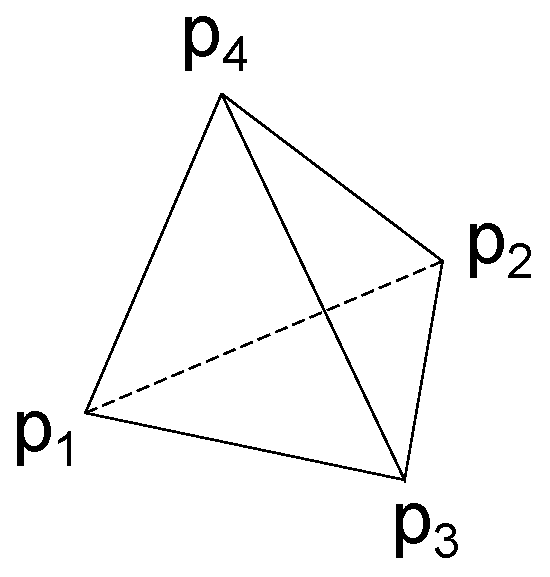
\includegraphics[width=0.25\linewidth]{figures/unit_tetrahedron.eps}
    \caption{Regular tetrahedron with labeled vertices.}
    \label{fig:unit_tetrahedron}
\end{figure}

The location and orientation of the regular tetrahedron depends on the particular space group of the cubic unit cell. For all space groups of interest, candidate tetrahedron barycenter coordinates $c$ are tabulated in Table \ref{table:tet_locations} assuming Cartesian axis-aligned cubic unit cells with unity edge length. Without loss of generality, only barycenters with coordinates all in the range $[0, 1)$ are listed. In addition, several barycenters may yield the same tetrahedron unit cell due to the symmetry of the cubic cell; in this case, only one barycenter is listed. For each barycenter point, there are two possible tetrahedrons that may be used to generate the tetrahedron unit cell because the regular tetrahedron is self dual. The first one has vertices defined by:
\begin{equation}
    \begin{split}
        p_1 & = c + (m, -m, -m) \\
        p_2 & = c + (-m, m, -m) \\
        p_3 & = c + (-m, -m, m) \\
        p_4 & = c + (m, m, m)
    \end{split}
\end{equation}
where $m$ is some positive value. If the desired tetrahedron edge length is given by $a$, then setting $m=\frac{a\sqrt{2}}{4}$ will yield a tetrahedron with the edge length $a$. The dual tetrahedron has vertices defined by:
\begin{equation}
    \begin{split}
        p_1 & = c + (-m, m, m) \\
        p_2 & = c + (m, m, -m) \\
        p_3 & = c + (m, -m, m) \\
        p_4 & = c + (-m, -m, -m)
    \end{split}
\end{equation}

\begin{table}
\caption{Location of tetrahedron barycenters for various cubic space groups.}
\label{table:tet_locations}
\centering
\begin{tabular}{c c} 
 \hline\hline
 Space group & Barycenter $c$ \\ 
 \hline\hline
 215 ($P\overline{4}3m$) & (0, 0, 0) \\
 & $(0.5, 0.5, 0.5)$ \\
 \hline
 216 ($F\overline{4}3m$) & (0, 0, 0) \\
 & (0.25, 0.25, 0.25) \\
 & (0.5, 0.5, 0.5) \\
 & (0.75, 0.75, 0.75) \\
 \hline
 217 ($I\overline{4}3m$) & (0, 0, 0) \\
 \hline
 221 ($Pm\overline{3}m$) & (0, 0, 0) \\
 & (0.5, 0.5, 0.5) \\
 \hline
 224 ($Pn\overline{3}m$, origin at $\overline{4}3m$) & (0, 0, 0) \\
 & (0.5, 0.5, 0.5) \\
 \hline
 224 ($Pn\overline{3}m$, origin at $\overline{3}m$) & (0.25, 0.25, 0.25) \\
 & (0.75, 0.75, 0.75) \\
 \hline
 225 ($Fm\overline{3}m$) & (0, 0, 0) \\
 & (0.25, 0.25, 0.25) \\
 & (0.5, 0.5, 0.5) \\
 & (0.75, 0.75, 0.75) \\
 \hline
 227 ($Fd\overline{3}m$, origin at $\overline{4}3m$) & (0, 0, 0) \\
 & (0.25, 0.25, 0.25) \\
 & (0.5, 0.5, 0.5) \\
 & (0.75, 0.75, 0.75) \\
 \hline
 227 ($Fd\overline{3}m$, origin at $\overline{3}m$) &  (0.125, 0.125, 0.125) \\
 & (0.375, 0.375, 0.375) \\
 & (0.625, 0.625, 0.625) \\
 & (0.875, 0.875, 0.875) \\
 \hline
 229 ($Im\overline{3}m$) & (0, 0, 0) \\
 \hline
\end{tabular}
\end{table}

The tetrahedral unit cell should be composed of a single connected component for manufacturing reasons. The number of connected components can be found by considering the triangulated surface mesh of the tetrahedral unit cell as a graph and searching for connected nodes \cite{hopcroft1973algorithm}.

\subsubsection{Tetrahedron mesh of input domain}
Once a tetrahedron unit cell has been created, a tetrahedron mesh of the input domain needs to be created. There are numerous meshing algorithms to accomplish this, including Delaunay-based methods \cite{shewchuk1998tetrahedral,si2010constrained,si2015tetgen}, methods suitable for polygon soups \cite{hu2018tetrahedral,hu2020fast}, and methods utilizing a static universal background mesh \cite{kabaria2017universal}.

\subsubsection{Mapping unit tetrahedron lattice to tetrahedron mesh}
The unit tetrahedron lattice is mapped to every tetrahedron in the tetrahedron mesh of the input domain through an affine transformation:
\begin{equation}
    \label{eq:tet_mapping}
    \mathbf{x_b} = \mathbf{A_b} \left( \mathbf{A_a}^{-1} \left( \mathbf{x_a} - \mathbf{p_{4a}} \right) \right) + \mathbf{p_{4b}}
\end{equation}
where $\mathbf{x_a}$ is a point in the unit tetrahedron stencil, $\mathbf{x_b}$ is the corresponding mapped point in the mesh tetrahedron, $\mathbf{p_{4a}}$ is the vertex $\mathbf{p_4}$ in the unit tetrahedron, $\mathbf{p_{4b}}$ is the corresponding vertex in the mesh tetrahedron, and the matrix $\mathbf{A}$ is given by
\begin{equation}
    \label{eq:tet_mapping_matrix}
    \begin{split}
        \mathbf{A} = \begin{bmatrix}
            p_{1x} - p_{4x} & p_{2x} - p_{4x} & p_{3x} - p_{4x} \\
            p_{1y} - p_{4y} & p_{2y} - p_{4y} & p_{3y} - p_{4y} \\
            p_{1z} - p_{4z} & p_{2z} - p_{4z} & p_{3z} - p_{4z} \\
        \end{bmatrix}
    \end{split}
\end{equation}
For $\mathbf{A_a}$, the vertices in Equation \ref{eq:tet_mapping_matrix} refer to those in the unit tetrahedron while for $\mathbf{A_b}$, the vertices in Equation \ref{eq:tet_mapping_matrix} refer to those in the mesh tetrahedron. Every point in the unit tetrahedron stencil is mapped using Equation \ref{eq:tet_mapping} to a particular tetrahedron in the mesh. The process is repeated for every tetrahedron in the mesh until the entire tetrahedron mesh of the design space is populated with stencils.

\section{Results}

\section{Conclusion}

\printbibliography

\end{document}